\section{Desugaring}
\label{sec:desugar}

%\begin{figure}[t]
%{\eightpoint
%\begin{verbatim}
%  int->int filter IterationFilter() {
%
%      work push 1 pop 1{
%
%          int counter = iter();
%          ...
%
%      }
%  }
%\end{verbatim}
%\caption{Example of a StreamIt filter using the iteration keyword.\protect\label{fig:iter-filter-example}}}
%\end{figure}
%
%
%\begin{figure}[t]
%{\eightpoint	
%\begin{verbatim}
%  int->int filter IterationFilter() {
%
%      int __iterationCount = 0;      
%
%      work push 1 pop 1{
%
%          int counter = __iterationCount;
%          ...
%
%          __iterationCount++;
%
%      }
%  }
%\end{verbatim}
%\caption{Example of a StreamIt filter with the iteration keyword desugared.\protect\label{fig:desugar-filter-example}}}
%\end{figure}

%
%\begin{figure}[t!]
%\centering
%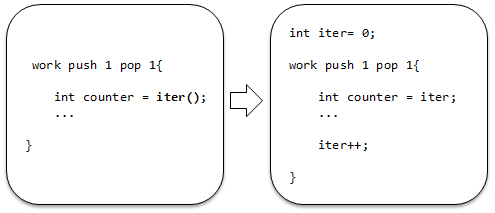
\includegraphics[width=3.3in]{figures/desugaring.png}
%\caption{Desugaring a filter using \texttt{iter()} keyword.\protect\label{fig:desugar}}
%\end{figure}


Under the StreamIt framework, filters are classified as iteration filters when there is use of the iteration keyword in its work function.  A simple lexer and parser can identify the use of this keyword, and it is represented accordingly in the intermediate representation.  To have it actually return the correct iteration value, we first convert the keyword to a compiler-usable construct.

{\tt iter()} is replaced with an access to a field holding the value of the iteration count.  The filter is given a definition for this field only if an {\tt iter()} use exists in its work or prework definition.  The work and prework function are appended with incrementing statements that update the iteration value.

The introduction of this iteration field creates state in the provided filter.  For future operations, the compiler does not consider this iteration field as part of the state of filter.  Future processes will maintain this inherent state without the downsides of introducing state.

It is important to note, these filters are not classified as stateful to the user, even though the filter is actually stateful on the iteration count after the desugaring process.  In classifying filters as stateful, the user is made aware of where data parallelism may be inhibited.  Iteration filters will not inhibit data parallelism because its state is identifiable to the compiler during the fission process.   

